\begin{figure}
  \centering
  \includegraphics[width=\linewidth]{fig/\conerfdirname/assets/update-attributes.pdf}
  \caption{{\bf Novel view and novel attribute synthesis on real data --}
    We synthesize scenes from a novel view and with a novel attribute
    combination, not seen during training.
    % \ky{
    A naive extension of HyperNeRF, HyperNeRF{+}$\pi$ fails to disentangle
    attributes and results in a modification of the scene irrespectively of
    attribute meaning \eg, opening mouth results in closing eyes at the same
    time.
    % is not what the attributes are describing--- and vice versa. 
    Ours-$\MaskNet$ improves the results, but does not disentangles the
    attribute space, as successfully done by our complete method.
    % results in entanglement.
    The differences between these methods can even lead to complete failure
    cases, as shown in the metronome and the toy car case.
  }
  % \cite{park2021hypernerf} with a projection network $\mathcal{A}$ to predict
  % attribute values $\{\attribute_\iAttribute\}$ causes that changes in the
  % output become entangled, \eg, opening the mouth also closes the
  % eyes.%causes closing eyes. }
  \label{fig:conerf-novel_view}
\end{figure}

\section{Results}
  \label{sec:conerf-results}

  \subsection{Datasets and baselines}

    We evaluate our method on two datasets: real video sequences captured with
    a smartphone ({\it real dataset}) and synthetically rendered sequences
    ({\it synthetic dataset}).
    Here we introduce those datasets and the baselines for our approach.

    \paragraph{Real dataset}
      % We evaluate our method on two types of data: real video sequences
      % captured with a smartphone and synthetically rendered sequences.
      Each of the seven real sequences is 1 minute long and was captured
      either with a Google Pixel 3a or an Apple iPhone 13 Pro.
      Four of them consists of people performing different facial expressions
      including smiling, frowning, closing or opening eyes, and opening mouth.
      % One of the four, we capture only the frontal view of the person, which
      % we reserve for the 2D image experiment.
      For the other three, we captured a toy car changing its shape ({\it
      a.k.a.
        }
      Transformer), a single metronome, and two metronomes beating with
      different rates.
      For one of the four videos depicting people, to use it for the 2D
      implementation case, we captured it with a static camera that shows a
      frontal view of the person.
      All other sequences feature camera motions showing front and sides of
      the object in the center of the scene.
      % \mk{One of the four videos depicting people is captured with a static
      % camera that shows a frontal view of the person, this video is reserved
      % for evaluating the 2D implementation of our method described in the
      % preceding section. All the remaining captures feature a moving camera
      % that captures the front and sides of the objects in the center of the
      % scene.}
      For videos with human subjects, the subjects signed a participant
      consent form, which was approved by a research ethics board.
      We informed the participants that their data will be altered with our
      method.

      We extract frames at 15 FPS which gives approximately 900 frames per
      capture.
      % \KY{do you mean every other frame is validation?}
      Because novel attribute synthesis via user control on real scenes does
      not have a ground truth view---we aim to create scenes with unseen
      attribute combinations---the benefit of our method is best seen
      qualitatively.
      Nonetheless, to quantitatively evaluate the rendering quality, we
      interpolate between two frames and evaluate its quality.
      In more detail, to minimize the chance of the dynamic nature of the
      scene interfering with this assessment, we use every other frame as a
      test frame for the interpolation task.

      % Annotations 
      For all human videos, we define three attributes---one for the status of
      each of the two eyes, and one for the mouth.
      We annotate only six frames per video in this case, specifically the
      frames that contain the extremes of each attribute (\eg, left eye fully
      open).
      For the toy car, we set the shape of the toy car to be an attribute, and
      annotate two extremes from two different view points---when the toy is
      in robot-mode and when it is in car-mode from its left and right side.
      For the metronomes, we consider the state of the pendulum to be the
      attribute and annotate the two frames with the two extremes for the
      single metronome case, and seven frames for the two metronome case as
      the pendulums of the two metronomes are often close to each other and
      required special annotations for these close-up cases;
      see~\cref{fig:conerf-novel_view}.

    \paragraph{Synthetic dataset}
      Since the lack of ground-truth data renders measuring the quality of
      novel attribute synthesis infeasible in practice, we leverage Kubric
      software~\cite{kubric2021github} to generate synthetic dataset, where we
      know exactly the state of each object in the scene.
      % is it is difficult to quantitatively measure novel attribute synthesis
      % with real data, we further use
      We create a simple scene where three 3D objects, the teapot
      \cite{teapot}, the Stanford bunny \cite{bunny}, and Suzanne
      \cite{suzanne}, are placed within the scene and are rendered with
      varying surface colors, which are our attributes;
      see~\cref{fig:conerf-kubric3d}.
      % We create one dataset that is in 3D for the NeRF experiments, and one
      % in 2D, using a top-view camera for the 2D tests. \KY{Below might
      % change---we might just to color changes ;)} \todo{% We move each object
      % in the scene independently of others on a predefined trajectory. }%
      We generate 900 frames for training and 900 frames for testing.
      To ensure that the attribute combination during training is not seen in
      the test scene, we set the attributes to be synchronized for the
      training split, and desynchronized for the test split.
      % \ky{
      We further render the test split from different camera positions than
      the training split to account for novel views.
      % }
      We randomly sample 5\% of the frames with a given attribute for each
      object to be set as the ground-truth attribute.
      During validation, we use attribute values directly to predict the
      image.

    \paragraph{Baselines}
      To evaluate the reconstruction quality of our method, CoNeRF, we compare
      it with four different baselines: \CIRCLE{1}~standard
      NeRF~\cite{mildenhall2020nerf}; \CIRCLE{2}~NeRF+Latent, a simple
      extension to NeRF where we concatenate each coordinate $\bx$ with a
      learnable latent code $\bbeta$ to support appearance changes of the
      scene; \CIRCLE{3}~Nerfies \cite{park2020deformable}; and
      \CIRCLE{4}~HyperNeRF\footnote{We use the version with dynamic plane
      slicing as it consistently outperforms the axis-aligned strategy; see
      \cite{park2021hypernerf} for more details.
      }~\cite{park2021hypernerf}.
      % \ky{
      Additionally, as existing methods do not support attribute-based control
      with a few-shot supervision, we create another baseline \CIRCLE{5} by
      extending HyperNeRF with a simple linear regressor $\pi$ that regresses
      $\bbeta_c$ given $\balpha_c$.
      We call this baseline HyperNeRF{+}$\pi$.
      % } \ky{ We also compare our approach against a %setting with disabled
      % mask part of our %pipeline. } slightly re-written
      To further show the importance of masking, we also compare our approach
      against a stripped-down version of our method, Ours{-}$\MaskNet $, where
      we disable the part of our pipeline responsible for masking.
      All baselines that utilize annotations were trained with the same sparse
      labels as our method.
      % \MK{is the above sentence I added true?} Ours{-}$\MaskNet$ to show its
      % importance.\tom{this sounds like some weird ablation study description}
      % \ky{} where we use $\mathcal{A}$ and $\mathcal{G}$ modules instead of
      % $\mathcal{H}$ (see \cref{fig:laced-implicit}). In short, we project
      % $\bbeta$ with an MLP, supervise the obtained representation with
      % annotations and use it as the latent representation that is processed
      % as in HyperNeRF \cite{park2021hypernerf}. We refer to this baseline as
      % HyperNeRF{+}Proj.

  \subsection{Comparison with the baselines}
    \begin{figure}
  \centering
  \begin{subfigure}[b]{0.164\linewidth}
    \centering
    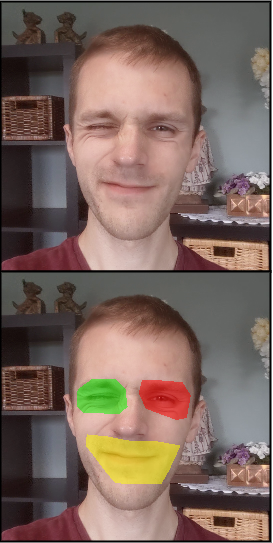
\includegraphics[width=\linewidth]{fig/\conerfdirname/assets/annotate/input.png}
    \caption{annotation}
  \end{subfigure}
  \hfill{}
  \begin{subfigure}[b]{0.816\linewidth}
    \centering
    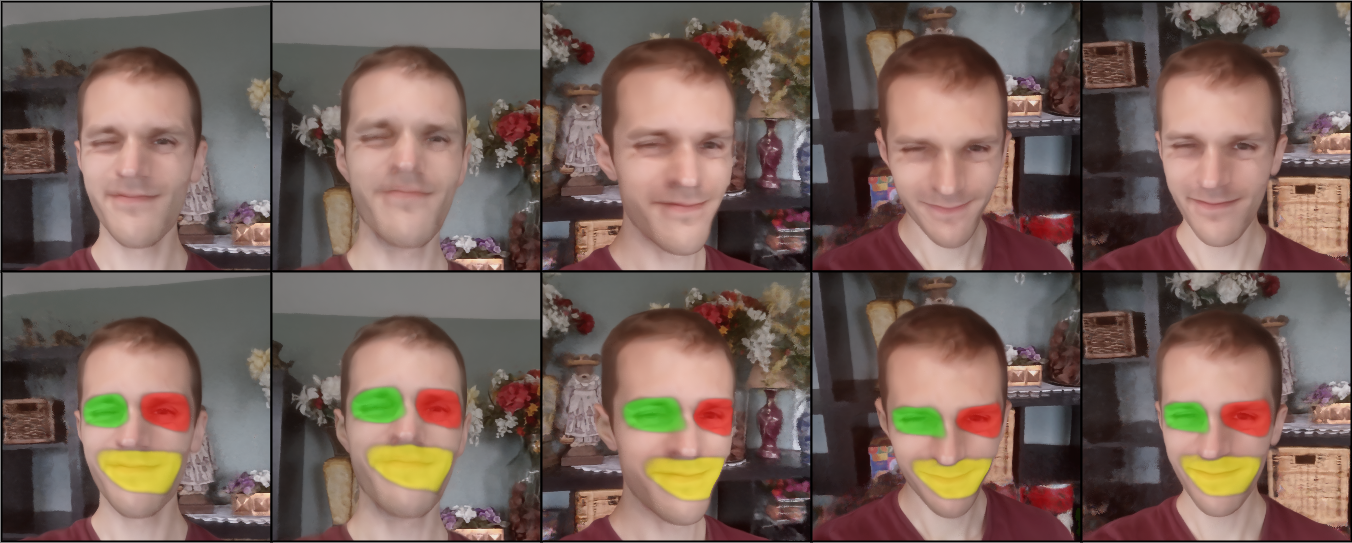
\includegraphics[width=\linewidth]{fig/\conerfdirname/assets/annotate/novel-views.png}
    \caption{unannotated views}
  \end{subfigure}
  \caption{{\bf Annotation example -- }
    We provide only a rough annotation for each attribute, which is enough for
    the method to discover the mask for each attribute across all views
    automatically.
    Bottom row shows masks overlaid on the image.
  }
  \label{fig:conerf-annotate}
\end{figure}

    \paragraph{Qualitative highlights}
      % \ky{%
      We first show qualitative examples of novel attribute and view synthesis
      on the real dataset in \cref{fig:conerf-novel_view}.
      Our method allows for controlling the selected attribute without
      changing other aspects of the image---our control is disentangled.
      This disentanglement allows our method to generate images with attribute
      combinations that were not seen at training time.
      % Our method allows to independently control multiple attributes without
      % the risk of entangling them with each other. In the case of
      % HyperNeRF{+}$\pi$, a simple regression strategy is unable to
      % disentangle the motions that happen within the scene which results in
      % uncontrollable rendering ({\it e.g.,} opening mouth triggered by
      % closing the eyes). 
      On the contrary, as there is no incentive for the learned embeddings of
      HyperNeRF to be disentangled, the simple regression strategy of
      HyperNeRF{+}$\pi$ results in entangled control, where when one tries to
      close/open the mouth it ends up affecting the eyes.
      % \KY{This might need rewrite after Fig3 is finalized}.
      The same phenomenon happens also for Ours{-}$\MaskNet$.
      % is unable to produce a distentangled representation as evidenced by
      % issues like the mouth opening when only the attribute responsible for
      % one of the eyes is modified.
      Moreover, due to the complexity of motions in the scene,
      HyperNeRF{+}$\pi$ fails completely to render novel views of the toy car,
      whereas our method, with only four annotated frames, successfully
      provides both controllability and high-quality renderings.
      % }%
      Please also see \SupplementaryMaterial for more qualitative results,
      including a video demonstration.

      Note that in all of these sequences, we provide highly sparse
      annotations and yet our method learns how each attribute should
      influence the appearance of the scene.
      In \cref{fig:conerf-annotate}, we show an example annotation and how the
      method finds the mask for unannotated views.

      \begin{figure}
  \centering
  \includegraphics[width=0.8\linewidth]{fig/\conerfdirname/assets/kubric3d/synthetic.pdf}
  \caption{{\bf Novel view and novel attribute synthesis on synthetic data -- }
    We show examples of novel view and novel attribute synthesis on synthetic
    data.
    The scene is composed of three objects, where the color of each object is
    their attribute.
    Our method provides control over the color of each object independently,
    whereas both HyperNeRF{+}$\pi$ and Ours{-}$\MaskNet$ fail to deliver
    controllability and results in all three objects having the same attribute
    in the rendered scene.
  }
  \label{fig:conerf-kubric3d}
\end{figure}
      \begin{figure}
  \centering
  \includegraphics[width=0.8\linewidth]{fig/\conerfdirname/assets/kubric3d/synthetic.pdf}
  \caption{{\bf Novel view and novel attribute synthesis on synthetic data -- }
    We show examples of novel view and novel attribute synthesis on synthetic
    data.
    The scene is composed of three objects, where the color of each object is
    their attribute.
    Our method provides control over the color of each object independently,
    whereas both HyperNeRF{+}$\pi$ and Ours{-}$\MaskNet$ fail to deliver
    controllability and results in all three objects having the same attribute
    in the rendered scene.
  }
  \label{fig:conerf-kubric3d}
\end{figure}
    \paragraph{Quantitative results on synthetic dataset}
      To complete the qualitative evaluation of our method, we provide results
      using synthetic dataset with available ground truth.
      We measure Peak Signal-to-Noise Ratio (PSNR), Multi-scale Structural
      Similarity (MS-SSIM)~\cite{wang2003multiscale}, and Learned Perceptual
      Image Patch Similarity (LPIPS)~\cite{zhang2018unreasonable} and report
      them in~\cref{tab:conerf-kubric3d}.
      With only 5\% of the annotations, our method provides the best
      novel-view and novel-attribute synthesis results, as reconfirmed by the
      qualitative examples in~\cref{tab:conerf-kubric3d}.
      As shown, neither HyperNeRF{+}$\pi$ nor Ours{-}$\MaskNet$ is able to
      provide good results in this case, as without disentangled control of
      each attribute, the novel attribute and view settings of each test frame
      cannot be synthesized properly.

    \paragraph{Interpolation task}
      To further verify that our rendering quality does not degrade with the
      introduction of controllability, we evaluate our method on a frame
      interpolation task without any attribute control.
      Unsurprisingly, as shown in~\cref{tab:conerf-sota}, all methods that
      support dynamic scenes work similarly, including ours for interpolation.
      Note that for the interpolation task, we interpolate every other frame,
      in order to minimize the chance of attributes affecting the evaluation.
      Here, we are purely interested in the rendering quality from a novel
      view.

      \begin{table}
  \centering
  \begin{tabular}{@{}lccc@{}}
    \toprule
    Method                     & PSNR $\uparrow$ & MS-SSIM $\uparrow$ & LPIPS $\downarrow$ \\
    \midrule
    NeRF                       & 28.795          & 0.951              & 0.210              \\
    NeRF + Latent              & 32.653          & 0.981              & 0.182              \\
    NeRFies                    & 32.274          & 0.981              & 0.180              \\
    HyperNeRF                  & 32.520          & 0.981              & 0.169              \\
    \midrule
    \textbf{Ours}{-}$\MaskNet$ & 32.061          & 0.979              & 0.167              \\
    \textbf{Ours}              & 32.342          & 0.981              & 0.168              \\

    \bottomrule
  \end{tabular}
  \caption{
    \textbf{Quantitative results (interpolation) -- }
    We report results in terms of PSNR, MS-SSIM, and LPIPS for the
    interpolation task.
    These results are obtained for interpolated view synthesis only, not for
    novel attribute rendering.
    Our method provides similar performance in terms of rendering quality, but
    with controllability.
  } % \caption
  \label{tab:conerf-sota}
\end{table}

      \begin{figure}
  \centering
  \includegraphics[width=0.8\linewidth, trim=0 320 0 0, clip]{fig/\conerfdirname/assets/face.pdf}
  \caption{
    {\bf 2D image generation example -- }
    Our framework also generalizes to direct generation of 2D images.
    Here we show novel attribute synthesis for a webcam video of a person
    making expressions.
    Each individual part of the scene is correctly controlled according to the
    attribute values.
  }
  % }
  \label{fig:conerf-2d-interpolation}
\end{figure}
  \subsection{Direct 2D rendering}
    To verify how our approach generalizes beyond NeRF models and volume
    rendering, we apply our method to videos taken from a single view point,
    creating a 2D rendering task.
    We show in~\cref{fig:conerf-2d-interpolation} a proof-of-concept for
    employing our approach outside of NeRF applications to allow controllable
    neural generative models.

  \subsection{Ablation study}
    \begin{table}
  \centering
  \normalsize
  \setlength{\tabcolsep}{2pt}
  \begin{tabular}{@{}lccc ccc@{}}
    \toprule
          & \multicolumn{3}{c}{Real (interpolation)} & \multicolumn{3}{c}{Synthetic (novel view \& attr.)}                                                                                  \\
    \cmidrule(lr){2-4}
    \cmidrule(lr){5-7}
    Model & PSNR $\uparrow$ & MS-SSIM $\uparrow$ & LPIPS $\downarrow$ & PSNR
    $\uparrow$ & MS-SSIM $\uparrow$ & LPIPS $\downarrow$ \\ \midrule Base
    ($\loss{recon}$) & 32.457 & 0.981 & 0.168 & 24.407 & 0.718 & 0.173 \\
    $+\loss{enc}$ & 32.478 & 0.982 & 0.167 & 27.018 & 0.871 & 0.164 \\ $+
    \loss{enc} +\loss{attr}$ & 32.254 & 0.981 & 0.167 & 27.322 & 0.873 & 0.147
    \\ $+ \loss{enc} + \loss{attr} +\loss{mask}$ & 32.342 & 0.981 & 0.168 &
    \textbf{32.394} & \textbf{0.972} & \textbf{0.139}\\
    \bottomrule\end{tabular} \caption{ \textbf{{Effect of loss functions --}}
    We report the rendering quality of our method as we procedurally introduce
    the loss terms.
    % < \resizebox 
    For controlled rendering with novel views and attributes (synthetic data),
    each loss term adds to the rendering quality, with the $\loss{mask}$ being
    critical.
    For the novel view rendering on real data, addition of loss functions for
    controllability do not have a significant effect on the rendering
    quality---they do no harm.
  } % \caption
  \label{tab:conerf-ablations}
\end{table}
    \paragraph{Loss functions}
      In~\cref{tab:conerf-ablations}, we show how each loss term affects the
      network's performance, contributing to performance improvements.
      When rendering novel views with novel attributes, the full formulation
      is a must, as without all loss terms the performance drops
      significantly---for example, results without $\loss{mask}$ is similar to
      Ours-$\MaskNet$ results in~\cref{tab:conerf-kubric3d} and
      \cref{fig:conerf-kubric3d}.
      In the case of the interpolation task, the additional loss functions for
      controllability have no significant effect on the rendering quality.
      In other words, our controllability losses \textbf{do not interfere}
      with the rendering quality, other than imbuing the framework with
      controllability.
      \vspace{-0.2em}

      \begin{figure}
  \centering
  \includegraphics[width=\linewidth]{fig/\conerfdirname/assets/annotations-differences.pdf}
  \caption{{\bf Effect of annotation quality -- }
    Our method is moderately robust to the quality of annotations.
    We visualize the results for two expressions: frowning and smiling, while
    keeping both eyes in a neutral position.
    Even with wildly varying annotations as shown, the reconstructions are
    reasonably controlled, with the exception of the top row, where we show a
    case where the annotations is too restrictive, resulting in the annotation
    being ignored for one eye.
    We show in bottom row also an interesting case, where the mask is large
    enough to start capturing the correlation among mouth expressions and the
    eye.
  }
  \label{fig:conerf-ablation_annotate}
\end{figure}
    \paragraph{Quality of few shot supervision}
      We test how sensitive our method is against the quality of annotation
      supervision.
      In~\cref{fig:conerf-ablation_annotate} we demonstrate how each
      annotation leads to the final rendering quality.
      Our framework is robust to a moderate degree to the inaccuracies in the
      annotations.
      However, when they are too restrictive, the mask may collapse, as shown
      on the top row.
      Too large of a mask could also lead to moderate entanglement of
      attributes, as shown in the bottom row.
      Still, in all cases, our method provides a reasonable control over what
      is annotated.

      % not using primes (not canonicalized parameters)
\begin{figure}
  \centering
  \begin{subfigure}[t]{0.38\linewidth}
    \centering
    \includegraphics[width=\linewidth]{fig/\conerfdirname/assets/beta-importance-annotations.pdf}
    \caption{annotated samples}
  \end{subfigure}
  \hfill{}
  \begin{subfigure}[t]{0.595\linewidth}
    \centering
    \includegraphics[width=\linewidth]{fig/\conerfdirname/assets/beta-importance-preds.pdf}
    \caption{renderings}
  \end{subfigure}
  \caption{{\bf Example with unannotated attributes --}
    We show an example of how our method performs when a part of the image
    changes appearance, but is not annotated.
    With the annotations in (a), we synthesize the scene with novel view and
    attributes in (b), where the two rows are with different $\bbeta$
    configurations.
    We denote the attribute configuration on the top of each column in (b).
    As shown, the change that is not annotated is simply encoded in the
    per-image encoding $\bbeta$.
  }
  \label{fig:conerf-ablation_unannotated}
\end{figure}
    \paragraph{Unannotated attributes}
      A natural question to ask is then what happens with the unannotated
      changes that may exist in the scene.
      In~\cref{fig:conerf-ablation_unannotated} we show how the method
      performs when annotating only parts of the appearance change within the
      scene.
      The unannotated changes of the scene get encoded as $\bbeta$, as in the
      case of HyperNeRF~\cite{park2021hypernerf}.
